\documentclass[aspectratio=169]{beamer}
\usetheme{Madrid}
\usecolortheme{seahorse}
\usefonttheme{professionalfonts}
\usepackage[utf8]{inputenc}
\usepackage{graphicx}
\usepackage{amsmath}
\usepackage{booktabs}
\usepackage{tikz}
\usepackage{fontawesome5}
\usepackage{lmodern}
\usepackage{hyperref}
\usepackage{microtype} % Melhora a justificação e reduz overfull

% Reduzir margens para evitar overfull em títulos longos
\setbeamersize{text margin left=5pt, text margin right=5pt}
\setbeamerfont{frametitle}{size=\small}
\setbeamerfont{title}{size=\normalsize}

% Cores personalizadas
\definecolor{cefetblue}{RGB}{0,51,102}
\definecolor{cefetgray}{RGB}{230,230,230}
\setbeamercolor{frametitle}{fg=white,bg=cefetblue}
\setbeamercolor{title}{fg=white,bg=cefetblue}
\setbeamercolor{block title}{fg=white,bg=cefetblue}
\setbeamercolor{block body}{bg=cefetgray,fg=black}
\setbeamercolor{item}{fg=cefetblue}

% Rodapé personalizado
\setbeamertemplate{footline}{
  \leavevmode%
  \hbox{%
  \begin{beamercolorbox}[wd=.8\paperwidth,ht=2.5ex,dp=1ex,left]{author in head/foot}%
    \usebeamerfont{author in head/foot}\hspace{1em}\insertshortauthor
    \hspace{2em}\insertshorttitle
  \end{beamercolorbox}%
  \begin{beamercolorbox}[wd=.2\paperwidth,ht=2.5ex,dp=1ex,right]{date in head/foot}%
    \insertframenumber{} / \inserttotalframenumber
    \hspace{1em}
    \raisebox{-0.5ex}{
\includegraphics[height=2ex]{../img/logo_cefet.png}}
  \end{beamercolorbox}}%
  \vskip0pt%
}

% Remove barra de navegação
\setbeamertemplate{navigation symbols}{}

% Sumário automático
\AtBeginSection[]{
  \begin{frame}{Sumário}
    \tableofcontents[currentsection, hideothersubsections]
  \end{frame}
}

\title[Sistemas Fuzzy Mamdani e Takagi-Sugeno]{Sistemas Fuzzy Mamdani e Takagi-Sugeno}
\author[Leonardo V. Guimarães]{Leonardo Vieira Guimarães}
\institute[CEFET-MG]{Pós-Graduação em Engenharia Elétrica, CEFET-MG}
\date{\today}

\begin{document}

\begin{frame}
    \titlepage
\end{frame}

\begin{frame}{Sumário}
    \tableofcontents
\end{frame}

\begin{frame}{Contexto e Motivação}
    \begin{itemize}
        \item Ambientes fechados exigem controle eficiente de ventilação para conforto térmico e economia de energia.
        \item Sistemas fuzzy permitem decisões flexíveis e interpretáveis, mesmo com incertezas e subjetividade.
        \item Dois paradigmas fuzzy: \textbf{Mamdani} (qualitativo) e \textbf{Takagi-Sugeno} (quantitativo/aproximação).
    \end{itemize}
    \vspace{0.5em}
    \centering
    % Imagem removida pois não está disponível
    % \includegraphics[width=0.45\linewidth,keepaspectratio]{../img/ambiente_ventilacao.png}
    % \begin{block}{\centering\small\color{red}%
    %     \textbf{Atenção:} Imagem \texttt{../img/ambiente\_ventilacao.png} não encontrada.\\
    %     Inclua o arquivo na pasta \texttt{img} para exibir corretamente.
    % }
    % \end{block}
\end{frame}

\begin{frame}{Objetivos}
    \begin{itemize}
        \item Desenvolver um sistema fuzzy Mamdani para controle de ventilação em ambientes fechados.
        \item Implementar um sistema Takagi-Sugeno para aproximação de funções não lineares.
        \item Analisar o impacto de funções de pertinência, operadores e técnicas de defuzzificação/otimização.
        \item Comparar desempenho, interpretabilidade e aplicações de cada abordagem.
    \end{itemize}
\end{frame}

\begin{frame}{Fluxo Geral dos Sistemas Fuzzy}
    \centering
    % Corrija o erro do TikZ: não use 'right=of ...', use posicionamento manual com 'at'
    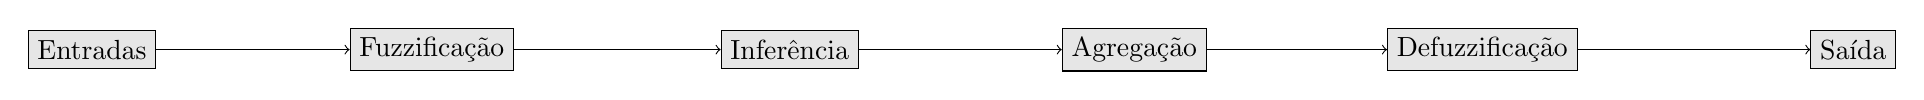
\begin{tikzpicture}[auto]
        \node[draw, rectangle, fill=cefetgray] (input) {Entradas};
        \node[draw, rectangle, fill=cefetgray] (fuzz) at ([xshift=3.5cm]input.east) {Fuzzificação};
        \node[draw, rectangle, fill=cefetgray] (inferencia) at ([xshift=3.5cm]fuzz.east) {Inferência};
        \node[draw, rectangle, fill=cefetgray] (agreg) at ([xshift=3.5cm]inferencia.east) {Agregação};
        \node[draw, rectangle, fill=cefetgray] (defuzz) at ([xshift=3.5cm]agreg.east) {Defuzzificação};
        \node[draw, rectangle, fill=cefetgray] (output) at ([xshift=3.5cm]defuzz.east) {Saída};
        \draw[->] (input) -- (fuzz);
        \draw[->] (fuzz) -- (inferencia);
        \draw[->] (inferencia) -- (agreg);
        \draw[->] (agreg) -- (defuzz);
        \draw[->] (defuzz) -- (output);
    \end{tikzpicture}
    \vspace{1em}
    \begin{itemize}
        \item \textbf{Mamdani:} saída fuzzy, defuzzificação obrigatória.
        \item \textbf{Takagi-Sugeno:} saída numérica direta (ordem zero/primeira ordem).
    \end{itemize}
\end{frame}

\section{Sistema Mamdani}

\begin{frame}{Sistema Mamdani: Controle de Ventilação}
    \begin{block}{Entradas}
        \begin{itemize}
            \item Temperatura interna ($15^\circ$C a $35^\circ$C)
            \item Umidade relativa (20\% a 100\%)
            \item Número de pessoas (0 a 20)
        \end{itemize}
    \end{block}
    \begin{block}{Saída}
        \begin{itemize}
            \item Intensidade da ventilação: fraca, moderada, forte (0 a 10)
        \end{itemize}
    \end{block}
    \begin{block}{Características}
        \begin{itemize}
            \item Funções de pertinência: triangulares
            \item Base de regras: 9 regras baseadas em conforto térmico
            \item Operadores: AND (mínimo), OR (máximo, soma)
            \item Defuzzificação: Centroide, Média do Máximo, Bissetriz
        \end{itemize}
    \end{block}
\end{frame}

\begin{frame}{Particionamento dos Universos de Discurso}
    \begin{columns}
        \column{0.5\textwidth}
        \textbf{Temperatura:}
        \begin{itemize}
            \item Baixa: 15 a 22
            \item Média: 18 a 30
            \item Alta: 25 a 35
        \end{itemize}
        \textbf{Umidade:}
        \begin{itemize}
            \item Baixa: 20 a 45
            \item Média: 35 a 85
            \item Alta: 70 a 100
        \end{itemize}
        \column{0.5\textwidth}
        \textbf{Pessoas:}
        \begin{itemize}
            \item Poucas: 0 a 7
            \item Moderado: 3 a 17
            \item Muitas: 12 a 20
        \end{itemize}
        \textbf{Ventilação:}
        \begin{itemize}
            \item Fraca: 0 a 4
            \item Moderada: 2 a 8
            \item Forte: 6 a 10
        \end{itemize}
    \end{columns}
\end{frame}

\begin{frame}{Funções de Pertinência - Mamdani}
    \begin{block}{}
        \centering
        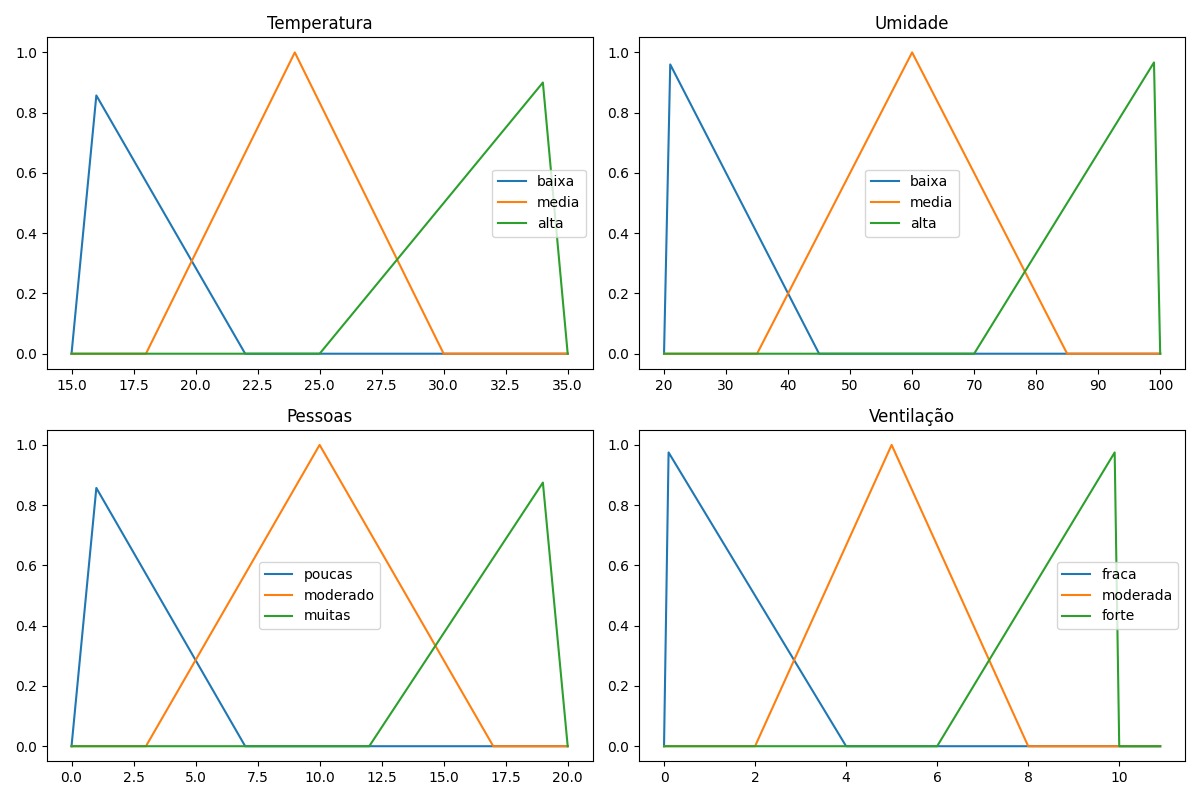
\includegraphics[width=0.75\linewidth,keepaspectratio]{../img/funcoes_pertinencia_mamdani2.png}
        \vspace{0.5em}
        \small Funções de pertinência das variáveis do sistema Mamdani.
    \end{block}
\end{frame}

\begin{frame}{Base de Regras Fuzzy - Mamdani}
    \begin{itemize}
        \item Se temperatura \textbf{alta} OU umidade \textbf{alta} OU pessoas \textbf{muitas} então ventilação \textbf{forte}
        \item Se temperatura \textbf{média} E umidade \textbf{média} E pessoas \textbf{moderado} então ventilação \textbf{moderada}
        \item Se temperatura \textbf{baixa} E umidade \textbf{baixa} E pessoas \textbf{poucas} então ventilação \textbf{fraca}
        \item Se temperatura \textbf{alta} E umidade \textbf{baixa} então ventilação \textbf{moderada}
        \item Se temperatura \textbf{média} E pessoas \textbf{muitas} então ventilação \textbf{forte}
        \item Se umidade \textbf{alta} E pessoas \textbf{poucas} então ventilação \textbf{moderada}
        \item Se temperatura \textbf{baixa} OU umidade \textbf{baixa} então ventilação \textbf{fraca}
        \item Se pessoas \textbf{moderado} E umidade \textbf{média} então ventilação \textbf{moderada}
        \item Se temperatura \textbf{média} E umidade \textbf{alta} então ventilação \textbf{forte}
    \end{itemize}
    \vspace{0.5em}
    \textit{Operadores: AND = mínimo, OR = máximo/soma}
\end{frame}

\begin{frame}{Exemplo de Inferência Fuzzy (Cenário 1)}
    \begin{itemize}
        \item \textbf{Entradas:} temperatura=28, umidade=80, pessoas=15
        \item \textbf{Fuzzificação:}
        \begin{itemize}
            \item temp\_media(28) $\approx$ 0.33, temp\_alta(28) $\approx$ 0.30
            \item umid\_alta(80) $\approx$ 0.33
            \item pess\_muitas(15) $\approx$ 0.37
        \end{itemize}
        \item \textbf{Regras ativadas:} R1, R2, R5, R8, R9
        \item \textbf{Agregação:} máximo das saídas das regras ativadas
        \item \textbf{Defuzzificação:} centroide, média do máximo, bissetriz
    \end{itemize}
\end{frame}

\begin{frame}{Superfície Fuzzy - Mamdani}
    \begin{block}{}
        \centering
        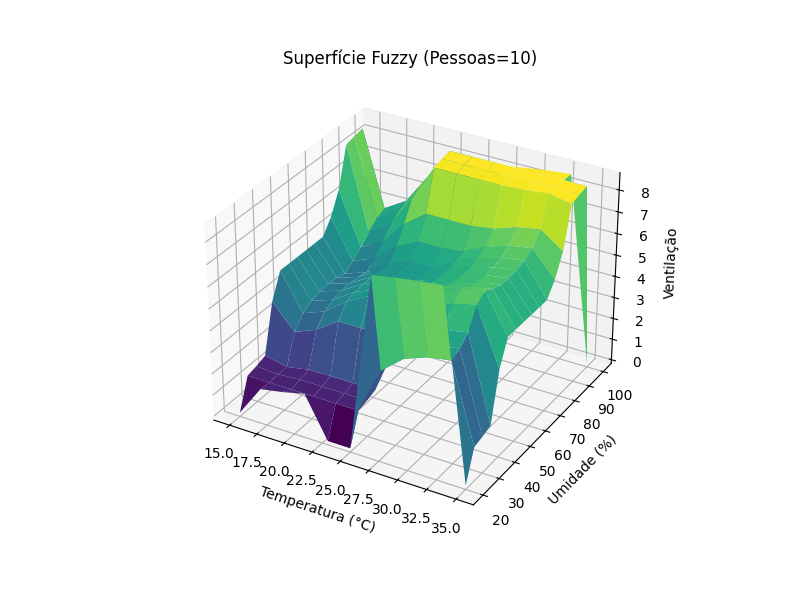
\includegraphics[width=0.75\linewidth,keepaspectratio]{../img/superficie_fuzzy_pessoas10_mamdani2.png}
        \vspace{0.5em}
        \small Superfície fuzzy: ventilação em função de temperatura e umidade (pessoas=10).
    \end{block}
\end{frame}

\begin{frame}{Saída Fuzzy Agregada - Mamdani}
    \begin{block}{}
        \centering
        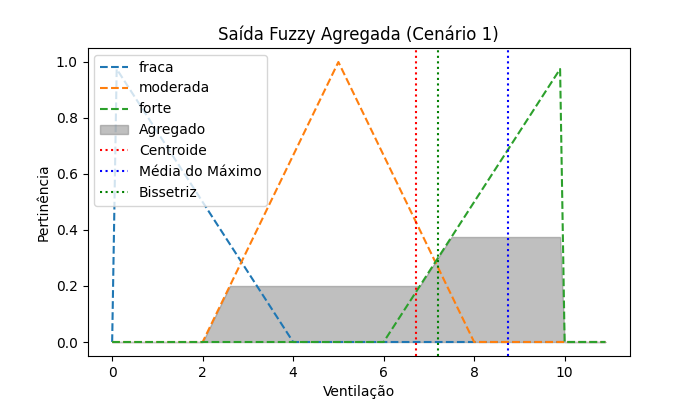
\includegraphics[width=0.75\linewidth,keepaspectratio]{../img/saida_fuzzy_cenario1_mamdani2.png}
        \vspace{0.5em}
        \small Saída fuzzy agregada e defuzzificação para o cenário 1.
    \end{block}
\end{frame}

\begin{frame}{Resultados Mamdani: Comparação de Técnicas}
    \begin{table}[h]
    \centering
    \begin{tabular}{|c|c|c|c|}
    \hline
    Cenário & Centroide & Média do Máximo & Bissetriz \\
    \hline
    1 & forte & forte & forte \\
    2 & moderada & moderada & moderada \\
    3 & fraca & fraca & fraca \\
    4 & forte & forte & forte \\
    5 & forte & forte & forte \\
    \hline
    \end{tabular}
    \end{table}
    \vspace{0.5em}
    \small Diferenças pequenas entre técnicas de defuzzificação. Sistema flexível e interpretável.
\end{frame}

\section{Sistema Takagi-Sugeno}

\begin{frame}{Sistema Takagi-Sugeno: Aproximação de Função}
    \begin{block}{Função alvo}
        $f(x) = e^{-x/5} \cdot \sin(3x) + 0.5 \cdot \sin(x)$, $x \in [0, 10]$
    \end{block}
    \begin{itemize}
        \item 3 regras (Baixo, Médio, Alto)
        \item Funções de pertinência: Gaussianas (centros 2, 5, 8), Triangulares, Trapezoidais
        \item Consequentes: Constantes (ordem zero) e lineares (primeira ordem)
        \item Otimização: Gradiente descendente para consequentes
    \end{itemize}
\end{frame}

\begin{frame}{Fluxo do Sistema Takagi-Sugeno}
    \begin{enumerate}
        \item Fuzzificação da entrada $x$ (cálculo das pertinências)
        \item Avaliação das regras: cada regra retorna $y_i = c_i$ (ordem zero) ou $y_i = a_i x + b_i$ (primeira ordem)
        \item Agregação: média ponderada das saídas das regras pelas pertinências
        \item Saída numérica direta (não fuzzy)
    \end{enumerate}
    \vspace{0.5em}
    \centering
    % Imagem removida pois não está disponível
    % \includegraphics[width=0.5\linewidth,keepaspectratio]{../img/fluxo_ts.png}
    \begin{block}{\centering\small\color{red}%
        \textbf{Atenção:} Imagem \texttt{../img/fluxo\_ts.png} não encontrada.\\
        Inclua o arquivo na pasta \texttt{img} para exibir corretamente.
    }
    \end{block}
\end{frame}

\begin{frame}{Função Alvo e Pertinências - Takagi-Sugeno}
    \begin{block}{}
        \centering
        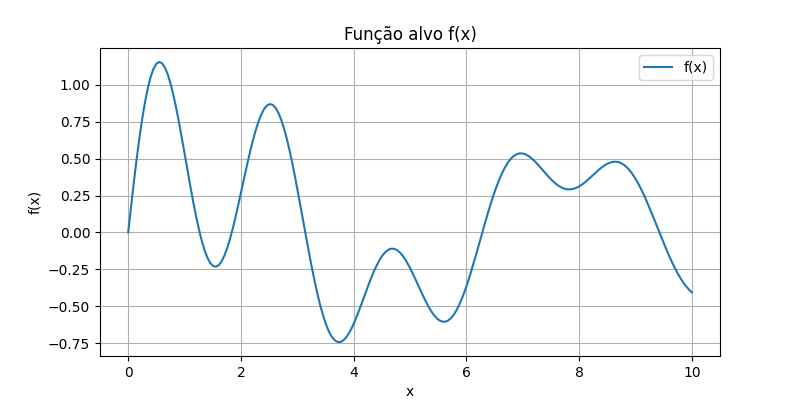
\includegraphics[width=0.75\linewidth,keepaspectratio]{../img/fx_takagi_sugeno2.png}
        \vspace{0.5em}
        \small Função alvo $f(x)$
    \end{block}
    \begin{block}{}
        \centering
        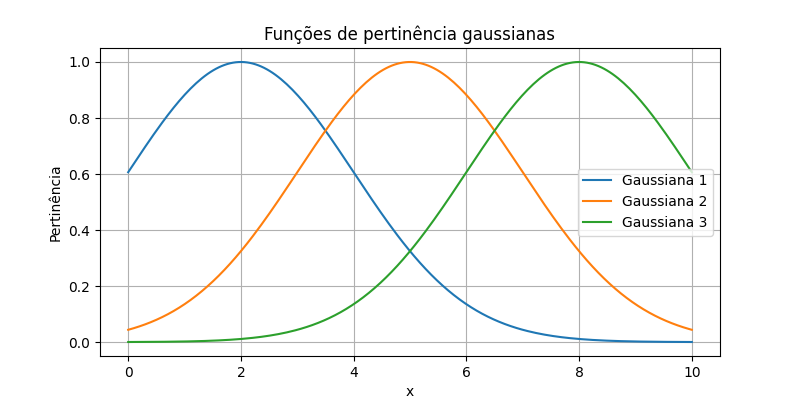
\includegraphics[width=0.75\linewidth,keepaspectratio]{../img/mfs_gauss_takagi_sugeno2.png}
        \vspace{0.5em}
        \small Funções de pertinência gaussianas
    \end{block}
\end{frame}

\begin{frame}{Aproximação Takagi-Sugeno: Resultados}
    \begin{block}{}
        \centering
        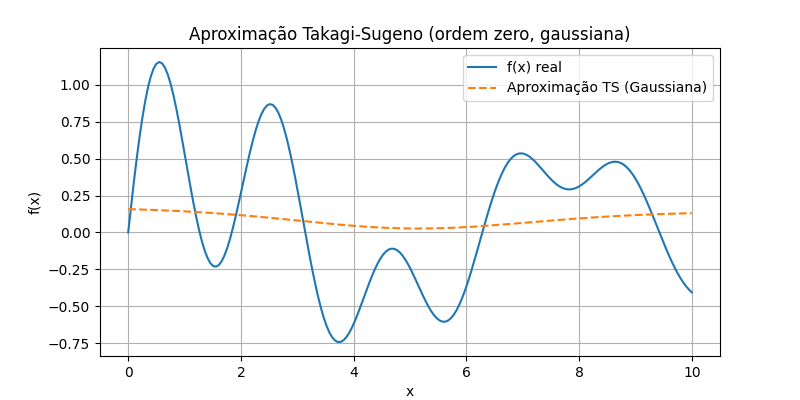
\includegraphics[width=0.75\linewidth,keepaspectratio]{../img/fx_aprox_gauss_takagi_sugeno2.png}
        \vspace{0.5em}
        \small Aproximação TS (ordem zero, gaussiana)
    \end{block}
    \begin{block}{}
        \centering
        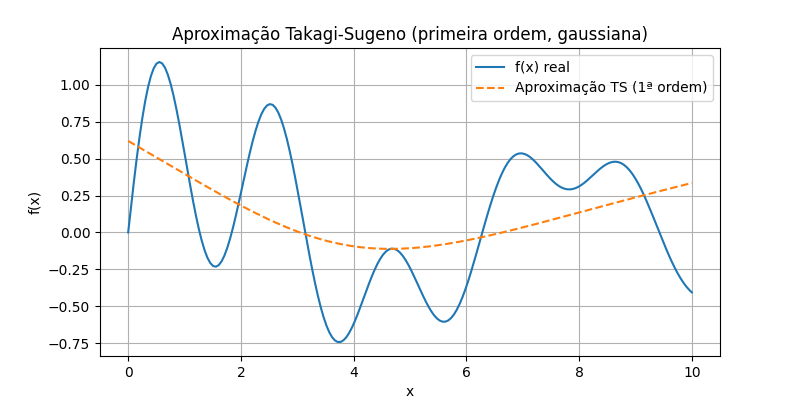
\includegraphics[width=0.75\linewidth,keepaspectratio]{../img/fx_aprox_1ordem_takagi_sugeno2.png}
        \vspace{0.5em}
        \small Aproximação TS (primeira ordem, gaussiana)
    \end{block}
\end{frame}

\begin{frame}{Comparação de Funções de Pertinência}
    \begin{block}{}
        \centering
        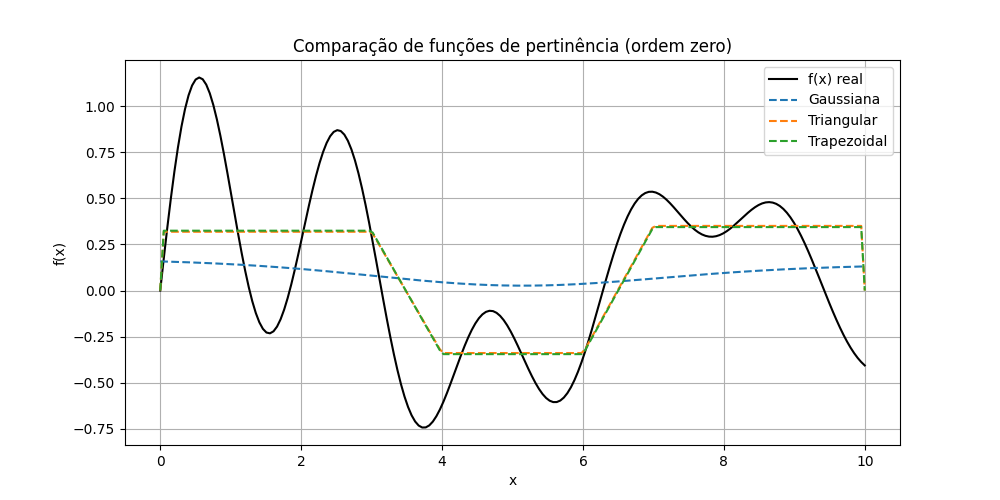
\includegraphics[width=0.75\linewidth,keepaspectratio]{../img/fx_aprox_comparacao_takagi_sugeno2.png}
        \vspace{0.5em}
        \small Comparação de funções de pertinência (ordem zero)
    \end{block}
\end{frame}

\begin{frame}{Otimização dos Consequentes}
    \begin{block}{}
        \centering
        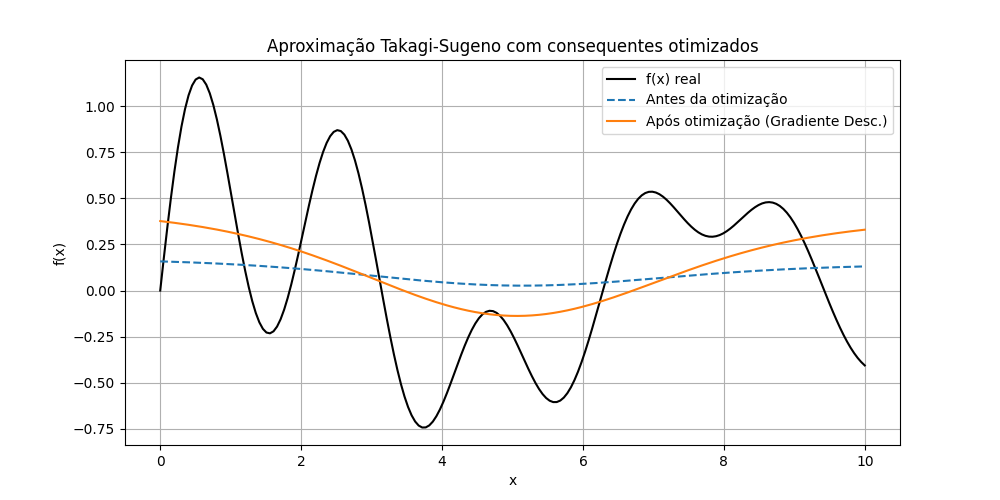
\includegraphics[width=0.75\linewidth,keepaspectratio]{../img/fx_aprox_otimizado_takagi_sugeno2.png}
        \vspace{0.5em}
        \small Aproximação TS com consequentes otimizados (gradiente descendente)
    \end{block}
\end{frame}

\begin{frame}{Erro de Aproximação}
    \begin{block}{}
        \centering
        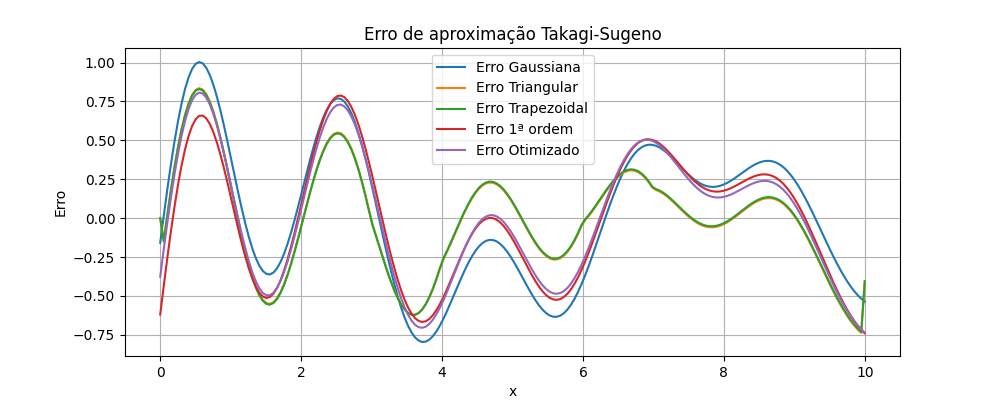
\includegraphics[width=0.75\linewidth,keepaspectratio]{../img/erro_takagi_sugeno2.png}
        \vspace{0.5em}
        \small Erro de aproximação para cada configuração
    \end{block}
\end{frame}

\begin{frame}{Quadro Comparativo: Mamdani vs Takagi-Sugeno}
    \begin{tabular}{|l|c|c|}
    \hline
    & \textbf{Mamdani} & \textbf{Takagi-Sugeno} \\
    \hline
    Saída & Qualitativa (fuzzy) & Numérica (precisa) \\
    Interpretação & Alta & Média/baixa \\
    Aplicação & Controle, decisão & Aproximação, modelagem \\
    Defuzzificação & Necessária & Não (ordem zero/1) \\
    Otimização & Não usual & Recomendada \\
    \hline
    \end{tabular}
\end{frame}

\begin{frame}{Principais Resultados}
    \begin{itemize}
        \item \textbf{Mamdani:} decisões qualitativas coerentes, diferenças pequenas entre técnicas de defuzzificação.
        \item \textbf{Takagi-Sugeno:} RMSE (ordem zero, gaussiana): $\approx$ 0.46; RMSE (triangular/trapezoidal): $\approx$ 0.35; RMSE otimizado: $\approx$ 0.41.
        \item Funções de pertinência e operadores influenciam o desempenho.
        \item Otimização dos consequentes reduz o erro de aproximação.
    \end{itemize}
\end{frame}

\begin{frame}{Discussão e Pontos-Chave}
    \begin{itemize}
        \item \textbf{Mamdani:} ideal para sistemas interpretáveis e decisões qualitativas.
        \item \textbf{Takagi-Sugeno:} excelente para modelagem e aproximação de funções complexas.
        \item Escolha de funções de pertinência, operadores e técnicas de otimização é fundamental.
        \item Sistemas fuzzy são flexíveis, adaptáveis e podem ser expandidos para aplicações reais.
    \end{itemize}
\end{frame}

\begin{frame}{Conclusões}
    \begin{itemize}
        \item Mamdani: eficaz para decisões qualitativas e interpretáveis.
        \item Takagi-Sugeno: aproxima funções não lineares com boa precisão, especialmente após otimização.
        \item A escolha das funções de pertinência e operadores influencia o desempenho.
        \item Sistemas fuzzy são ferramentas poderosas para controle e modelagem.
    \end{itemize}
\end{frame}

\begin{frame}{Sugestões para Trabalhos Futuros}
    \begin{itemize}
        \item Aplicar os sistemas fuzzy em dados reais de ambientes monitorados.
        \item Explorar sistemas fuzzy com múltiplas entradas e saídas.
        \item Investigar técnicas avançadas de otimização dos parâmetros fuzzy.
        \item Integrar os sistemas fuzzy a plataformas de automação residencial ou industrial.
    \end{itemize}
\end{frame}

\begin{frame}{Referências}
    \footnotesize
    \begin{itemize}
        \item Zadeh, L. A. (1965). Fuzzy sets.
        \item Mamdani, E. H., \& Assilian, S. (1975). An experiment in linguistic synthesis with a fuzzy logic controller.
        \item Takagi, T., \& Sugeno, M. (1985). Fuzzy identification of systems and its applications to modeling and control.
        \item Ross, T. J. (2010). Fuzzy Logic with Engineering Applications.
        \item Haykin, S. (2008). Neural Networks and Learning Machines.
    \end{itemize}
\end{frame}

\begin{frame}{Perguntas?}
    \centering
    \Huge \faQuestionCircle[regular] \\
    \vspace{1em}
    \Large Obrigado!
\end{frame}

\end{document}
